\chapter{Étude théorique et conception}
\section{Étude préliminaire:}
Les méthodes existantes pour l'analyse des sentiments peuvent être regroupées en deux catégories principales: méthodes basées sur la connaissance (knowledge-based), ou sur l'apprentissage automatique (machine learning). \\
\subsection{Méthodes basées sur la connaissance: }
Dans les méthodes basées sur la connaissance, également appelé classification des sentiments basée sur le lexique, l'objectif est de
construire ou utiliser des lexiques de mots de sentiments existants avec des étiquettes de sentiments indiquées pour les mots
ou les phrases dans le texte. La classification du texte est définie par des règles; une fonction sur les mots, comme la somme des polarités des mots \cite{taboada2011lexicon}. Cette approche ne nécessite pas
toute formation (autre que la formation d'un lexique, si nécessaire). \\

Hu, Minqing et Bing Liu \cite{hu2004mining} ont construit un lexique, utilisant uniquement WordNet (base de données lexicale) et une liste d'adjectifs de semences étiquetés. Cette liste contient uniquement des adjectifs positifs (par exemple, grand, étonnant, agréable, cool) et des adjectifs négatifs (par exemple, mauvais, ennuyeux). Leur méthode récupère et étiquette automatiquement les synonymes (même polarité) et antonymes (polarité opposée). Ce processus permet à la liste de devenir un lexique. Un inconvénient de cette approche est qu'elle n'est applicable que dans les langues où WordNet est disponible. Dans tous les cas, la méthode basée sur les connaissances peut être difficile en raison du bruit dans les données textuelles, tandis que la création manuelle de règles pour combiner des informations sur les mots obtenus à partir des lexiques de sentiments prend du temps et des efforts.\\
\subsection{Méthodes basées sur l'apprentissage automatique: }
D'autre part, l'apprentissage automatique nécessite de former un modèle pour prédire la polarité du texte. Le modèle est formé avec des messages texte, étiquetés pour leur sentiment et représentés comme des vecteurs de fonctionnalités. Ce dernier nécessite classiquement un prétraitement de texte à l'aide d'outils de traitement de langage comme NLTK6. Le prétraitement du texte implique principalement la tokenisation, le stemming, le balisage et éventuellement l'analyse du texte. La sélection des caractéristiques appropriées à partir des données est cruciale et s'est révélée être un problème majeur et est toujours un objectif clé pour les chercheurs.\\

Des travaux antérieurs sur l'analyse des sentiments ont exploité des méthodes bien connues d'apprentissage automatique (machine learning) supervisé, telles que Naive Bayes \cite{martinez2006learning}, SVMs \cite{vinet2011missing, ho1995random,wahid2017prestasi}. Des travaux plus récents utilisent des modèles d'apprentissage profond (deep learning) \cite{goldberg2017neural}, en particulier les réseaux neuronaux récurrents (RNN) et le réseau neuronal convolutionnel (CNN). Cette thèse porte également sur les modèles d'apprentissage profond.
\begin{figure}[H]
    \centering
    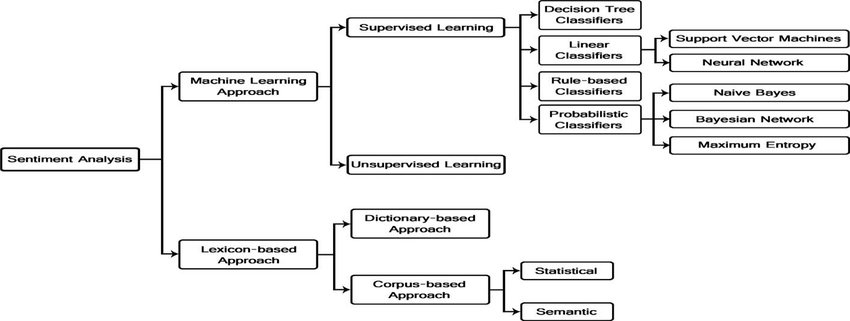
\includegraphics[width=\textwidth]{etude-theorique-conception/assets/sentiment-analysis-methods.jpg}
    \caption{Description des méthodes d'analyse des sentiments}
    \label{fig:my_label}
\end{figure}
\subsection{Limites des solutions existantes:}
Certaines limitations des solutions existantes de l'analyse des sentiments:
\begin{itemize}
    \item \textcolor{DispositionColor}{Pour les méthodes basées sur la connaissance:}
    \begin{itemize}
        \item Elles peuvent être difficile en raison du bruit dans les données textuelles, tandis que la création manuelle de règles pour combiner des informations sur les mots obtenus à partir des lexiques de sentiments prend du temps et des efforts.
        \item L'approche est qu'elle n'est applicable que dans les langues où le dictionnaire (La base de données lexicale) est disponible.
        \item Elles nécessitent de puissantes ressources linguistiques pour extraire des informations à partir des mots, chose qui n'existe pas toujours.
    \end{itemize}
    \item \textcolor{DispositionColor}{Pour les méthodes basées sur l'apprentissage automatique:}
    \begin{itemize}
        \item La sélection des caractéristiques appropriées à partir des données est cruciale et s'est révélée être un problème majeur et est toujours un objectif clé pour les chercheurs.
    \end{itemize}
\end{itemize}  
\section{NLP (Natural Language Processing):}
Le traitement du langage naturel est un sous-domaine de la linguistique, l'informatique, l'ingénierie de l'information et de l'intelligence artificielle concerné par les interactions entre les ordinateurs et les langues (naturelles) humaines, en particulier comment programmer des ordinateurs pour traiter et analyser de grandes quantités de données en langage naturel.\\

Les défis du traitement du langage naturel impliquent fréquemment la reconnaissance vocale, la compréhension du langage naturel et la génération du langage naturel.

\begin{figure}[H]
    \centering
    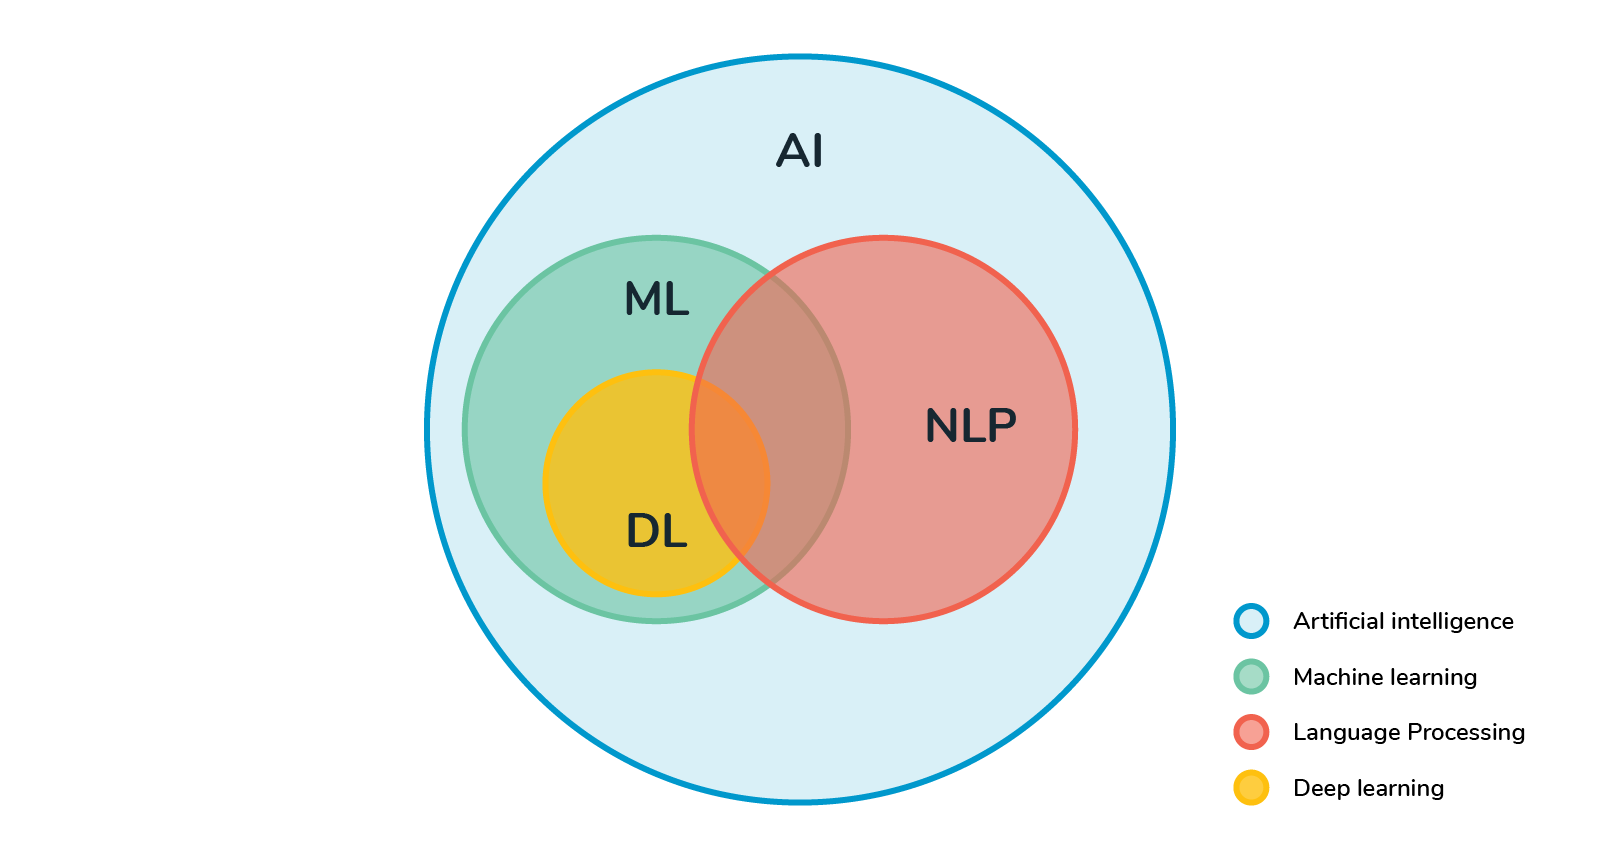
\includegraphics[width=\textwidth]{etude-theorique-conception/assets/nlp.png}
    \caption{NLP est une branche de l'intelligence artificielle}
    \label{fig:my_label}
\end{figure}

Ce qui suit est une liste des tâches les plus recherchées dans le traitement du langage naturel. Certaines de ces tâches ont des applications directes dans le monde réel, tandis que d'autres servent généralement de sous-tâches qui sont utilisées pour aider à résoudre des tâches plus importantes.\\

Bien que les tâches de traitement du langage naturel soient étroitement liées, elles sont fréquemment subdivisées en catégories pour plus de commodité:

\subsection{Syntaxe:}
\subsubsection{Induction grammaticale:}
La Génération d'une grammaire formelle qui décrit la syntaxe d'un langage. \\ \cite{klein2002natural}
\subsubsection{Lemmatisation:}
La tâche de supprimer uniquement les terminaisons flexionnelles et de renvoyer la forme de dictionnaire de base d'un mot qui est également connu sous le nom de lemme.
\subsubsection{Segmentation morphologique:}
La séparation des mots en morphèmes individuels et identifiez la classe des morphèmes. La difficulté de cette tâche dépend fortement de la complexité de la morphologie (c'est-à-dire la structure des mots) de la langue considérée.
\subsubsection{Segmentation des mots:}
La séparation d'un morceau de texte continu en mots séparés. Pour une langue comme l'anglais, c'est assez trivial, car les mots sont généralement séparés par des espaces. Cependant, certaines langues écrites ne marquent pas les limites des mots de cette manière, et dans ces langues, la segmentation du texte est une tâche difficile qui nécessite la connaissance du vocabulaire et de la morphologie des mots dans la langue.
\subsubsection{Catégorie grammaticale (Part-of-speech tagging):}
Cela implique d'identifier la catégorie grammaticale pour chaque mot.
\subsubsection{Analyse (Parsing):}
La détermination d'une arbre d'analyse (analyse grammaticale) d'une phrase donnée. La grammaire des langues naturelles est ambiguë et les phrases typiques ont de multiples analyses possibles. Peut-être de façon surprenante, pour une phrase typique, il peut y avoir des milliers d'analyses potentielles (dont la plupart sembleront complètement absurdes pour un humain).
\subsubsection{Rupture de phrase:}
Étant donné un morceau de texte, on trouve les limites de la phrase. Ces limites sont souvent marquées par des points ou d'autres signes de ponctuation, mais ces mêmes caractères peuvent servir à d'autres fins (par exemple, marquer des abréviations).
\subsubsection{"Stemming":}
Cela implique de couper les mots à leur forme racine.
\subsubsection{"Extraction terminologique":}
Le but de l'extraction terminologique est d'extraire automatiquement les termes pertinents d'un corpus donné.

\subsection{Sémantique:}
\subsubsection{Sémantique lexicale:}
La signification informatique des mots individuels dans leur contexte.
\subsubsection{Sémantique distributionnelle:}
L'apprentissage des représentations sémantiques à partir des données.
\subsubsection{Reconnaissance des entités nommées:}
Il s'agit de déterminer les parties d'un texte qui peuvent être identifiées et classées en groupes prédéfinis. Par exemple les noms de personnes et les noms de lieux.
\subsubsection{Désambiguïsation du sens des mots:}
Beaucoup de mots ont plus d'un sens; nous devons sélectionner le sens qui est le plus convenable au contexte. Pour ce problème, on reçoit généralement une liste de mots et de sens de mots associés, par exemple à partir d'un dictionnaire ou d'une ressource en ligne telle que WordNet.
\subsubsection{Extraction de relations:}
Étant donné un morceau de texte, on identifie les relations entre les entités nommées.
\subsubsection{Génération du langage naturel:}
Il s'agit d'utiliser des bases de données pour dériver des intentions sémantiques et les convertir en langage humain.
\subsection{Discours:}
\subsubsection{Synthèse automatique:}
La production d'un résumé lisible d'un morceau de texte.
\subsubsection{Résolution de coréférence:}
Étant donné une phrase ou un morceau de texte, on détermine quels mots (mentions) font référence aux mêmes objets (entités).
\subsection{Parole:}
\subsubsection{Reconnaissance de la parole:}
À partir d'un extrait sonore d'une ou de plusieurs personnes parlant, on détermine la représentation textuelle du discours.
\subsubsection{Segmentation de la parole:}
Étant donné un extrait sonore d'une ou de plusieurs personnes parlant, on le sépare en mots. Une sous-tâche de reconnaissance vocale et généralement regroupée avec elle.
\subsubsection{Synthèse de la parole à partir du texte (Text-to-speech)}
Étant donné un texte, on transforme ses unités et on produit une représentation parlée. La synthèse vocale peut être utilisée pour aider les gens avec une basse vision. \cite{yi2011assistive}


\begin{figure}[H]
    \centering
    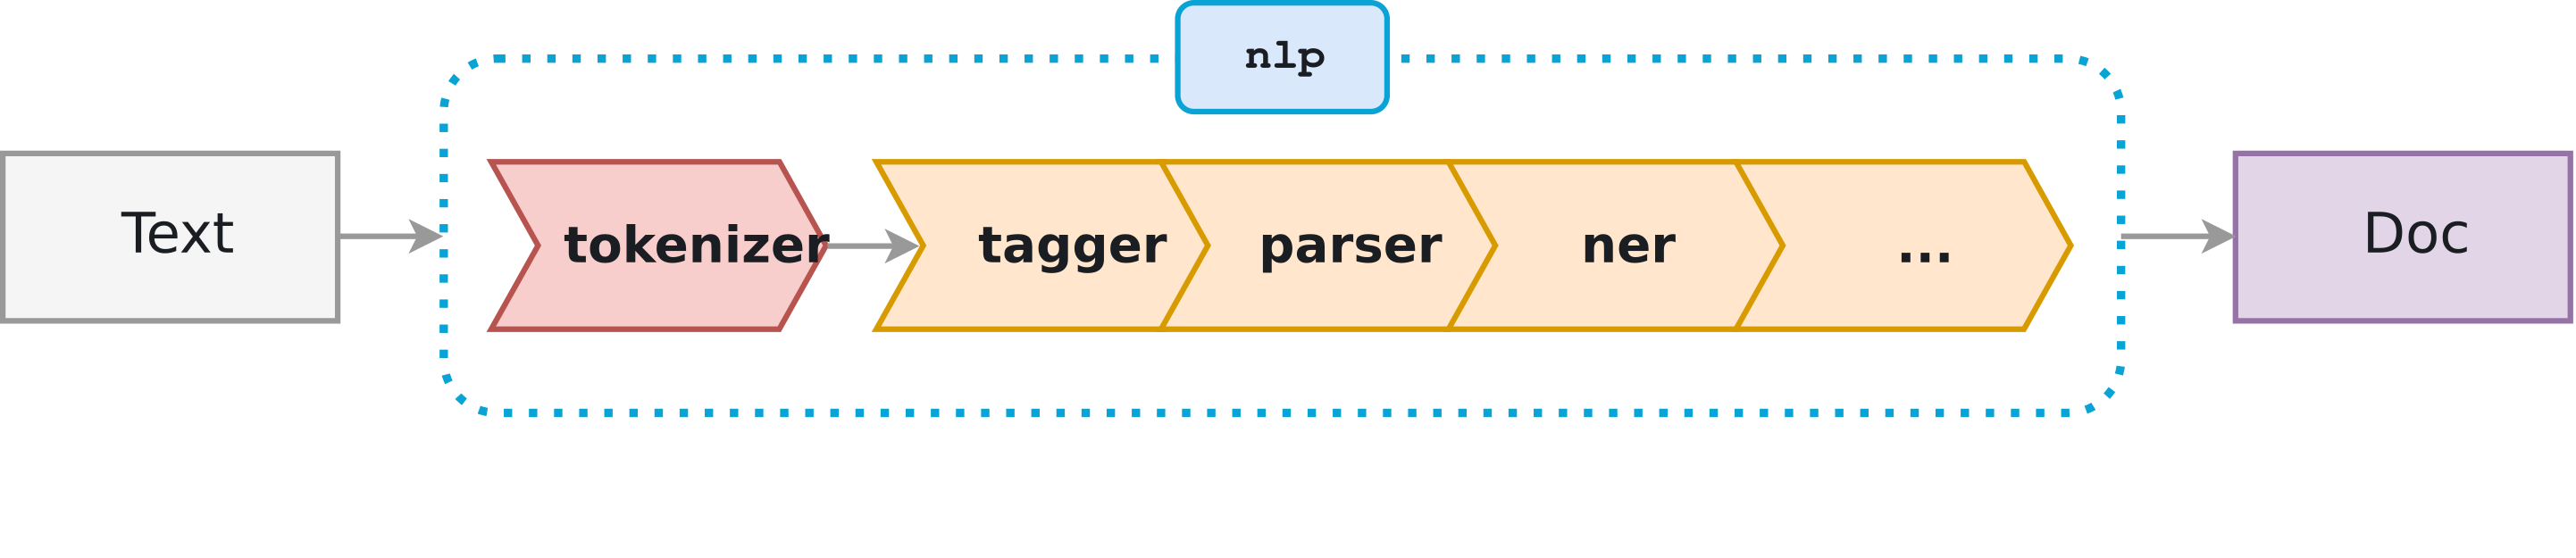
\includegraphics[width=\textwidth]{etude-theorique-conception/assets/nlp1.png}
    \caption{Processus NLP}
    \label{fig:my_label}
\end{figure}

\section{Algorithme Naive Bayes:}
L'algorithme Naive Bayes est un algorithme de classification probabiliste simple qui s'appuie sur le théorème de Bayes. Naive Bayes a des hypothèses d'indépendance fortes (naïves) entre les caractéristiques. En termes simples, un classificateur Naive Bayes suppose que la présence d'une caractéristique particulière dans une classe n'est pas liée à la présence de toute autre caractéristique. Par exemple, un ballon peut être considéré comme un ballon de football s'il est dur, rond et d'environ sept pouces de diamètre. Même si ces caractéristiques dépendent les unes des autres ou de l'existence des autres caractéristiques, Bayes naïf pense que toutes ces propriétés contribuent indépendamment à la probabilité que ce ballon soit un ballon de football, c'est pourquoi il est connu comme naïf. \\

Les modèles Naive Bayes sont faciles à construire. Ils sont également très utiles pour de très grands ensembles de données. Bien que les modèles Bayes naïfs soient simples, ils sont connus pour surpasser même les modèles de classification les plus sophistiqués. Parce qu'ils nécessitent également un temps de formation relativement court, ils constituent une bonne alternative pour une utilisation dans les problèmes de classification. \\

Résuméement, Bayes naïf est un modèle de probabilité conditionnel: étant donné une instance de problème à classer, représentée par un vecteur $x=x_{1},...,x_{n}$  représentant n fonctionnalités (variables indépendantes), il assigne à cette instance des probabilités ${p(C_{k}| x_{1},...,x_{n})}$ pour chaque $K$ résultats ou classes possibles ou classes $C_{k}$. \cite{murty2011pattern} \\

Le problème avec la formulation ci-dessus est que si le nombre d'entités n est grand ou si une entité peut prendre un grand nombre de valeurs, alors baser un tel modèle sur des tables de probabilités est irréalisable. Nous reformulons donc le modèle pour le rendre plus maniable. En utilisant le théorème de Bayes, la probabilité conditionnelle peut être décomposée comme:
\begin{equation}
    P(C_{k} | X)=\frac{P(X | C_{k}) P(C_{k})}{P(X)}
\end{equation}

En pratique, il n'y a d'intérêt que pour le numérateur de cette fraction, car le dénominateur ne dépend pas de $C$ et les valeurs des traits $x_ {i}$ sont données, de sorte que le dénominateur est effectivement constant. Le numérateur est équivalent au modèle de probabilité conjoint ${p(C_{k},x_{1},...,x_{n})}$ qui peut être réécrite comme suit, en utilisant la règle de chaîne de la définition de la probabilité conditionnelle:
\begin{equation}
    \begin{aligned}
    p\left(C_{k}, x_{1}, \ldots, x_{n}\right) &=p\left(x_{1}, \ldots, x_{n}, C_{k}\right) \\
    &=p\left(x_{1} | x_{2}, \ldots, x_{n}, C_{k}\right) p\left(x_{2}, \ldots, x_{n}, C_{k}\right) \\
    &=p\left(x_{1} | x_{2}, \ldots, x_{n}, C_{k}\right) p\left(x_{2} | x_{3}, \ldots, x_{n}, C_{k}\right) p\left(x_{3}, \ldots, x_{n}, C_{k}\right) \\
    &=\cdots \\
    &=p\left(x_{1} | x_{2}, \ldots, x_{n}, C_{k}\right) p\left(x_{2} | x_{3}, \ldots, x_{n}, C_{k}\right) \ldots p\left(x_{n-1} | x_{n}, C_{k}\right) p\left(x_{n} | C_{k}\right) p\left(C_{k}\right)
    \end{aligned}
\end{equation}

Maintenant, les hypothèses d'indépendance conditionnelle "naïve" entrent en jeu: supposons que toutes les fonctionnalités de $x$ sont mutuellement indépendantes, conditionnelles à la catégorie $C_{k}$, dans cette hypothèse, $
    p\left(x_{i} | x_{i+1}, \ldots, x_{n}, C_{k}\right)=p\left(x_{i} | C_{k}\right)
    $ \\

Ainsi, le modèle commun peut être exprimé comme: 
\begin{equation}
    \begin{aligned}
    p\left(C_{k} | x_{1}, \ldots, x_{n}\right) & \propto p\left(C_{k}, x_{1}, \ldots, x_{n}\right) \\
    &=p\left(C_{k}\right) p\left(x_{1} | C_{k}\right) p\left(x_{2} | C_{k}\right) p\left(x_{3} | C_{k}\right) \cdots \\
    &=p\left(C_{k}\right) \prod_{i=1}^{n} p\left(x_{i} | C_{k}\right)
    \end{aligned}
\end{equation}
où $\propto$ dénote la proportionnalité. \\

Cela signifie que sous les hypothèses d'indépendance ci-dessus, la distribution conditionnelle sur la variable de classe $C$ est: \\
\begin{center}
    $p\left(C_{k} | x_{1}, \ldots, x_{n}\right)=\frac{1}{Z} p\left(C_{k}\right) \prod_{i=1}^{n} p\left(x_{i} | C_{k}\right)$
\end{center}
où $Z=p(\mathbf{x})=\sum_{k} p\left(C_{k}\right) p\left(\mathbf{x} | C_{k}\right)$ $x_{1}, \ldots, x_{n}$ c'est-à-dire une constante si les valeurs des variables d'entité sont connues.
\paragraph{Construire un classificateur à partir du modèle de probabilité:}
Jusqu'à présent, la discussion a dérivé le modèle d'entité indépendant, c'est-à-dire le modèle de probabilité naïf de Bayes. Le classificateur naïf de Bayes combine ce modèle avec une règle de décision. Une règle courante consiste à choisir l'hypothèse la plus probable; il s'agit de la règle de décision maximale a posteriori ou MAP(maximum a posteriori). Le classificateur Bayes, est la fonction qui attribue une étiquette de classe ${\displaystyle {\hat{y}} = C_ {k}}$ pour certains $k$ comme suit: \\
\begin{center}
    $\hat{y}=\underset{k \in\{1, \ldots, K\}}{\operatorname{argmax}} p\left(C_{k}\right) \prod_{i=1}^{n} p\left(x_{i} | C_{k}\right)$  
\end{center}


\section{Vader:}
Vader (Valence Aware Dictionary and sentiment Reasoner) est un lexique et un outil d'analyse des sentiments basé sur des règles, qui est spécifiquement adapté aux sentiments exprimés dans les médias sociaux. Vader utilise une combinaison d'un lexique de sentiments qui est une liste de caractéristiques lexicales généralement étiquetées selon leur orientation sémantique comme positives ou négatives.\\

Vader s'est avéré très efficace dans le traitement de textes de médias sociaux, de critiques de films et de produits. Cela est dû au fait que Vader ne parle pas seulement du score de positivité et de négativité, mais nous indique également à quel point un sentiment est positif ou négatif (compound).\cite{hutto2014Vader}\\


\subsection{Quantifier l'émotion d'un mot:}
L'analyse des sentiments Vader s'appuie principalement sur un dictionnaire qui mappe les caractéristiques lexicales aux intensités émotionnelles appelées scores des sentiments. Le score de sentiment d'un texte peut être obtenu en résumant l'intensité de chaque mot dans le texte. Et par caractéristiques lexicales, on veut dire tout ce que nous utilisons pour la communication textuelle (mots, "emojis" au cas de l'analyse des tweets par exemple, acronymes...) \\

L'intensité d'émotion ou le score de sentiment est mesuré sur une échelle de -4 à +4, où -4 est le plus négatif et +4 est le plus positif. Le point médian 0 représente un sentiment neutre.\\

Vader construit son dictionnaire en utilisant les évaluateurs humains d'Amazon Mechanical Turk, et pour contrer la subjectivité des évaluateurs (notions différentes de ce qui est ositif ou negatif), les créateurs de Vader ont utilisé non seulement un, mais un certain nombre d'évaluateurs humains et ont fait la moyenne de leurs notes pour chaque mot. Cela repose sur le concept de la sagesse de la foule (the wisdom of the crowd).
\subsection{Quantifier l'émotion d'une phrase:}
L'analyse de sentiment Vader renvoie un score de sentiment compris entre -1 et 1, du plus négatif au plus positif en sommant les scores de sentiment de chaque mot de la phrase existant dans le dictionnaire Vader avant de normaliser cette somme pour le mapper à une valeur comprise entre -1 et 1. La normalisation utilisée par \cite{hutto2014Vader}: \\ 
\begin{center}
    $\frac{x}{\sqrt{x^{2}+\alpha}}$ 
\end{center}

$x$ est la somme des scores de sentiment des mots constitutifs de la phrase et $\alpha$ est un paramètre de normalisation que nous fixons à 15. La normalisation est représentée graphiquement ci-dessous.
\begin{figure}[H]
    \centering
    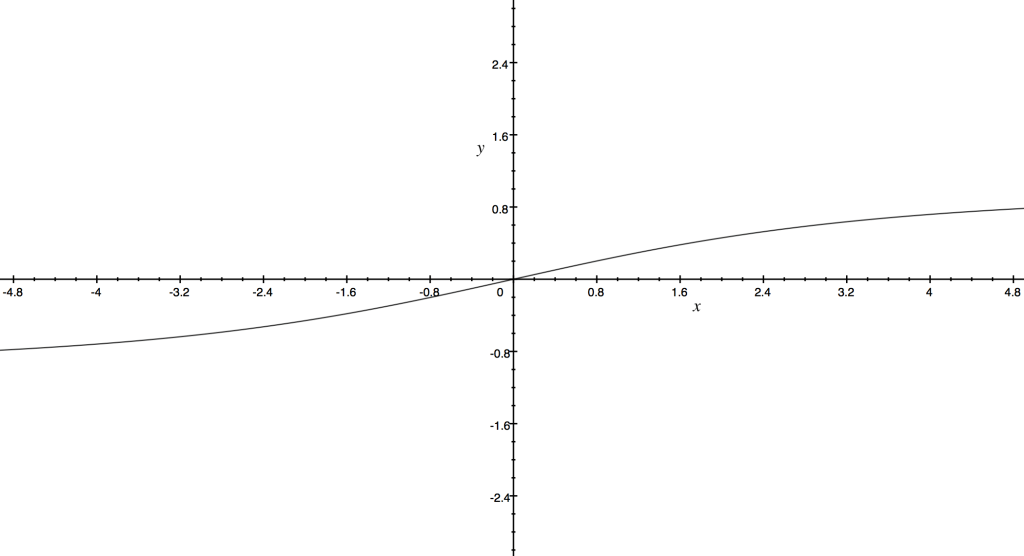
\includegraphics[width=0.6\textwidth]{etude-theorique-conception/assets/vader-normalization.png}
    \caption{Normalisation de Vader}
    \label{fig:my_label}
\end{figure}
Nous voyons ici que lorsque $x$ grandit, il devient de plus en plus proche de -1 ou 1. Pour un effet similaire, s'il y a beaucoup de mots dans le document auquel vous appliquez l'analyse des sentiments Vader, on obtient un score proche de -1 ou 1. Ainsi,l'analyse des sentiments Vader fonctionne mieux sur les documents courts, comme les tweets et les phrases, pas sur les gros documents.

\section{Conception du système:}
Dans cette étape, nous abordons la partie conception du projet, dans laquelle, nous
détaillons les différents éléments de conception, en commançant d'abord par spécificier les besoins fonctionnels de notre système, établir une architecture générale puis une modélisation statique du système à travers un diagramme de classes.
\subsection{Spécification des besoins fonctionnels:}
La spécification de ces besoins va nous permettre d’avoir une meilleure approche des utilisateurs, des fonctionnalités et de la relation entre les deux. Elle sera alors sous forme d'un diagramme de cas d’utilisation où on va procéder par l'identification des acteurs agissant sur notre système et les différentes cas d'utilisation: \\
\begin{figure}[H]
    \centering
    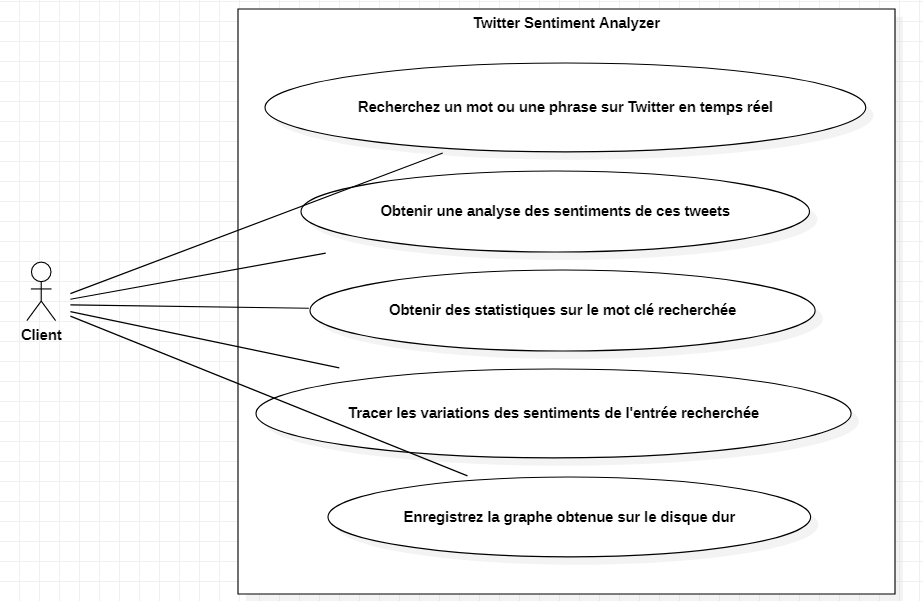
\includegraphics[width=\textwidth]{etude-theorique-conception/assets/useCase.png}
    \caption{Diagramme de cas d'utilisation}
    \label{fig:my_label}
\end{figure}
\subsection{Architecture générale de la solution:}
Pour réaliser notre système, on a choisi à suivre une architecture adapté à la nature de notre projet que nous représentons dans ce diagramme:
\begin{figure}[H]
    \centering
    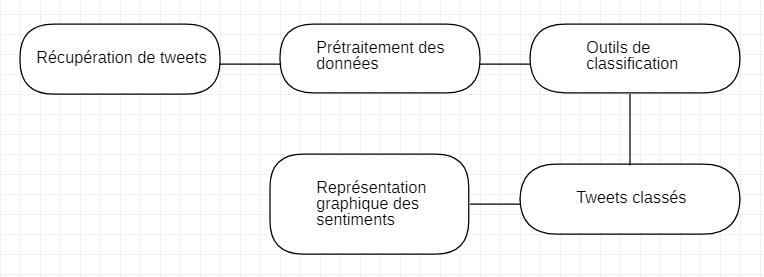
\includegraphics[width=\textwidth]{etude-theorique-conception/assets/architecture.png}
    \caption{Architecture du système}
    \label{fig:my_label}
\end{figure}
Comme on remarque dans le diagramme ci-dessus, on peut diviser le fonctionnement de notre application en cinque grandes parties:
\begin{itemize}
    \item \textcolor{DispositionColor}{Récupération de tweets:} La recherche et l'extraction des tweets contenant le mot clé entré par l'utilisateurs.
    \item \textcolor{DispositionColor}{Prétraitement des données:} Cette partie consiste à appliquer les différentes tâches et techniques de "NLP" pour traiter les tweets récupérés.
    \item \textcolor{DispositionColor}{Outils de classification:} Définir les méthodes suivies pour l'analyse de sentiments et la classification des tweets. 
    \item \textcolor{DispositionColor}{Tweets classés:} Classer ces tweets par des labels (positif ou négatif par exemple) et donner une évaluation générale sur l'ensemble de tweets récupérés.  
    \item \textcolor{DispositionColor}{Représentation graphique des sentiments:} Représentation graphique des sentiments de tweets selon les méthodes d'analyse choisie.
\end{itemize}
\subsection{Diagramme de classes:}
Le diagramme de classes est une modélisation statique du système en termes de classes et
de relations entre ces classes. Son intérêt réside dans la modélisation des entités du
système d'information.\\

Vu la nature de notre projet, nous avons décidé de créer deux entités illustrées dans le diagramme suivant:
\begin{figure}[H]
    \centering
    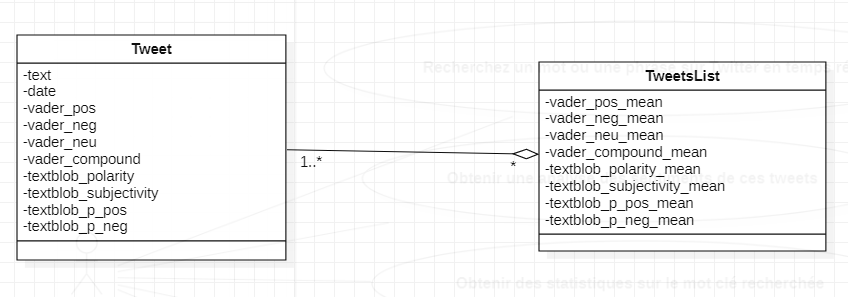
\includegraphics[width=\textwidth]{etude-theorique-conception/assets/classDiagram.png}
    \caption{Diagramme de classes}
    \label{fig:my_label}
\end{figure}
\begin{itemize}
    \item \textcolor{DispositionColor}{Tweet:} On utilise cette classe pour stocker les différentes informations liées à chaque tweet récupérés.
    \item \textcolor{DispositionColor}{TweetsList:} On utilise cette classe pour stocker les informations liées à l'ensemble de tweets récupérés.
\end{itemize}
\section{Conclusion:}
Dans ce chapitre, nous avons effectué une étude théorique où on a exploré les différents concepts utilisé pour la réalisation du projet, comme on a abordé le côté conceptuel du projet. 



